\section{Motivation}
\label{sec:intro:motivation}

In this section, we first examine the need for inductive biases in
machine learning. Then we analyze where current deep learning models
can get inductive biases from, and finally, we highlight some problems
that this dissertation addresses inductive biases for deep linguistic
structured prediction.

\subsection{Generalization: The Need for Inductive Bias}
\label{ssec:intro:need-of-bias}

Any system~(natural or artificial) that makes general inferences based
on particular and limited data must constrain its hypotheses
somehow. With limited observations and resources~(time, memory,
energy), our human intelligence of generalizing to new environments
makes us efficiently learn when interacting with the world and other
human beings. This efficiency largely depends on many inductive biases
from human intelligence~\citep{Gershman2021WhatMU}, which can
potentially be helpful for machine intelligence. According to
extensive cognitive science
studies~\citep{Spelke1990PrinciplesOO,Bienenstock1996CompositionalityMP,Rehder2003ACT,harlow1949formation,
  Lake2016BuildingMT,Gershman2021WhatMU}, there are many inductive
biases for human intelligence, such as compositionality, causality,
learning to learn, etc. We do not imply machine intelligence should
mimic human intelligence. Instead, we argue that those key human
inductive biases help overcome limited observations and resources that
may inspire us to design machine intelligence.

On the machine intelligence side, the no-free-lunch theorem for
machine learning~\citep{baxter2000model,wolpert1995no} tells us that
inductive biases that influence hypodissertation selection is necessary to
obtain generalization. \citet{mitchell1980need} argues that inductive
biases constitute the heart of generalization and, indeed a key basis
for learning itself.

\subsubsection{The Definition of Inductive Biases}
\label{sssec:intro:def-bias}
Let us examine a concrete example: the popular supervised learning
setting. We design algorithms that can learn from a set of supervised
training examples to predict a certain target output for an input. The
learning algorithm is presented with some training examples that
demonstrate the intended relationship between the input and output
values. Then the learner is supposed to learn a target function that
captures the correlations between the inputs and outputs. Furthermore,
we hope that the learned target function can approximate the correct
output, even for examples that have not been shown during training. We
call the ability to generalize unseen data a generalization. This
generalization problem cannot be solved without additional assumptions
since unseen situations might have an arbitrary output value. The kind
of necessary assumptions is subsumed in the phrase inductive bias.

%\begin{figure}[!th]
%\centering
%\includegraphics[width=0.80\textwidth]{supervised-learning-hypodissertation.pdf}
%\caption{\label{fig:intro-hypodissertation}Hypodissertation, Generatioalization in
%  Supervised Learning Setting\todo{Current fig is directly copied from
%    Ben Taskar's dissertation, redraw it}}
%\end{figure}

In this dissertation, following the definition of bias
in~\cite{mitchell1980need}, we define \kw{indutive bias} as:
\dquoted{Any bias for choosing one generalization over another, other
  than strict consistency with the observed training instances.}


\subsubsection{The Use of Inductive Biases}
\label{sssec:intro:use-bias}
As the definition stated above, inductive biases can be any assumption
beyond the observed training data. In this dissertation, we focused on the
supervised learning setting, where observed training data only means
the annotated training data directly available to that task. Inductive
biases are widely studied in the history of machine learning. In the
following, we list common ways of using inductive biases in
machine learning.

For the popular supervised learning setting, let $\mathcal{H}$ refer
to machine learning model families, including deep learning
models. Finding a target hypodissertation $h$ is reduced to estimating the
model parameters by fitting the training data. Hence, preferences
beyond training data can naturally be organized into two goals:
choosing the hypodissertation class $\mathcal{H}$ and finding the $h$ is
necessary to generalize to new data. For example, different \kw{model
  families} can represent different hypodissertation classes. For example,
generalized linear models, such as logistic regression and support
vector machines, can only support linear decision
boundaries. Secondly, inductive biases are also used in \kw{feature
  engineering}. For data that are not linear separable, the choices of
\kw{kernels design} also introduce inductive bias in kernel-based
SVM models. There are also many assumptions about optimization for
finding the specific hypodissertation $h$. For example, smoothness
assumptions in the \kw{optimization} method, such as Stochastic
gradient descent, were shown to have better
generalization. \kw{Inference Algorithms}, such as combinatorial
optimization approaches, such as graph cuts, partitions, bipartie
mactching, and dynamic programming can also be involved during the
hypodissertation learning, which will also constrain the learning. In this
dissertation, we mainly focus on representation learning. For
inference, we use methods, such as greedy search, maximum spanning
connected graph, and dynamic programming for CKY parsing. Finally, the
biases in the \kw{Training Data} will also influence the hypodissertation
finding. It is often the case that available datasets do not exactly
represent the data distribution of interest. One particularly
problematic case is when the dataset is biased against a particular
demographic group, which often leads to model predictions that
unfairly disadvantage members of that group. Hence, \kw{Data
  manipulation} can also help find the desired hypodissertation by
augmenting the original training data with inductive biases.

In this dissertation, we mainly use \kw{neural architectures} and \kw{data
  manipulation} to support our inductive biases for deep linguistic
structure prediction. To help understand the inductive biases, in
the following, we will first introduce two examples of inductive
biases used in the deep learning era, then we present the main study
the goal of using inductive biases for deep linguistic structured
prediction with independent factorization.

\subsection{Inductive Biases in Deep Learning}
\label{ssec:intro:bias-source}
According to the universal approximation
theorem~\citep{hornik1989multilayer}, a properly parameterized neural
network can represent any function. Furthermore, training data seems
rich enough for many tasks nowadays. It seems purely data-driven deep
learning can learn any target function. Then, what kind of inductive
biases do we need in the deep learning era? In the following, we show two
examples of inductive biases used in computer vision and natural
language processing in the deep learning era.

\begin{figure}[!tbp]
  \centering
  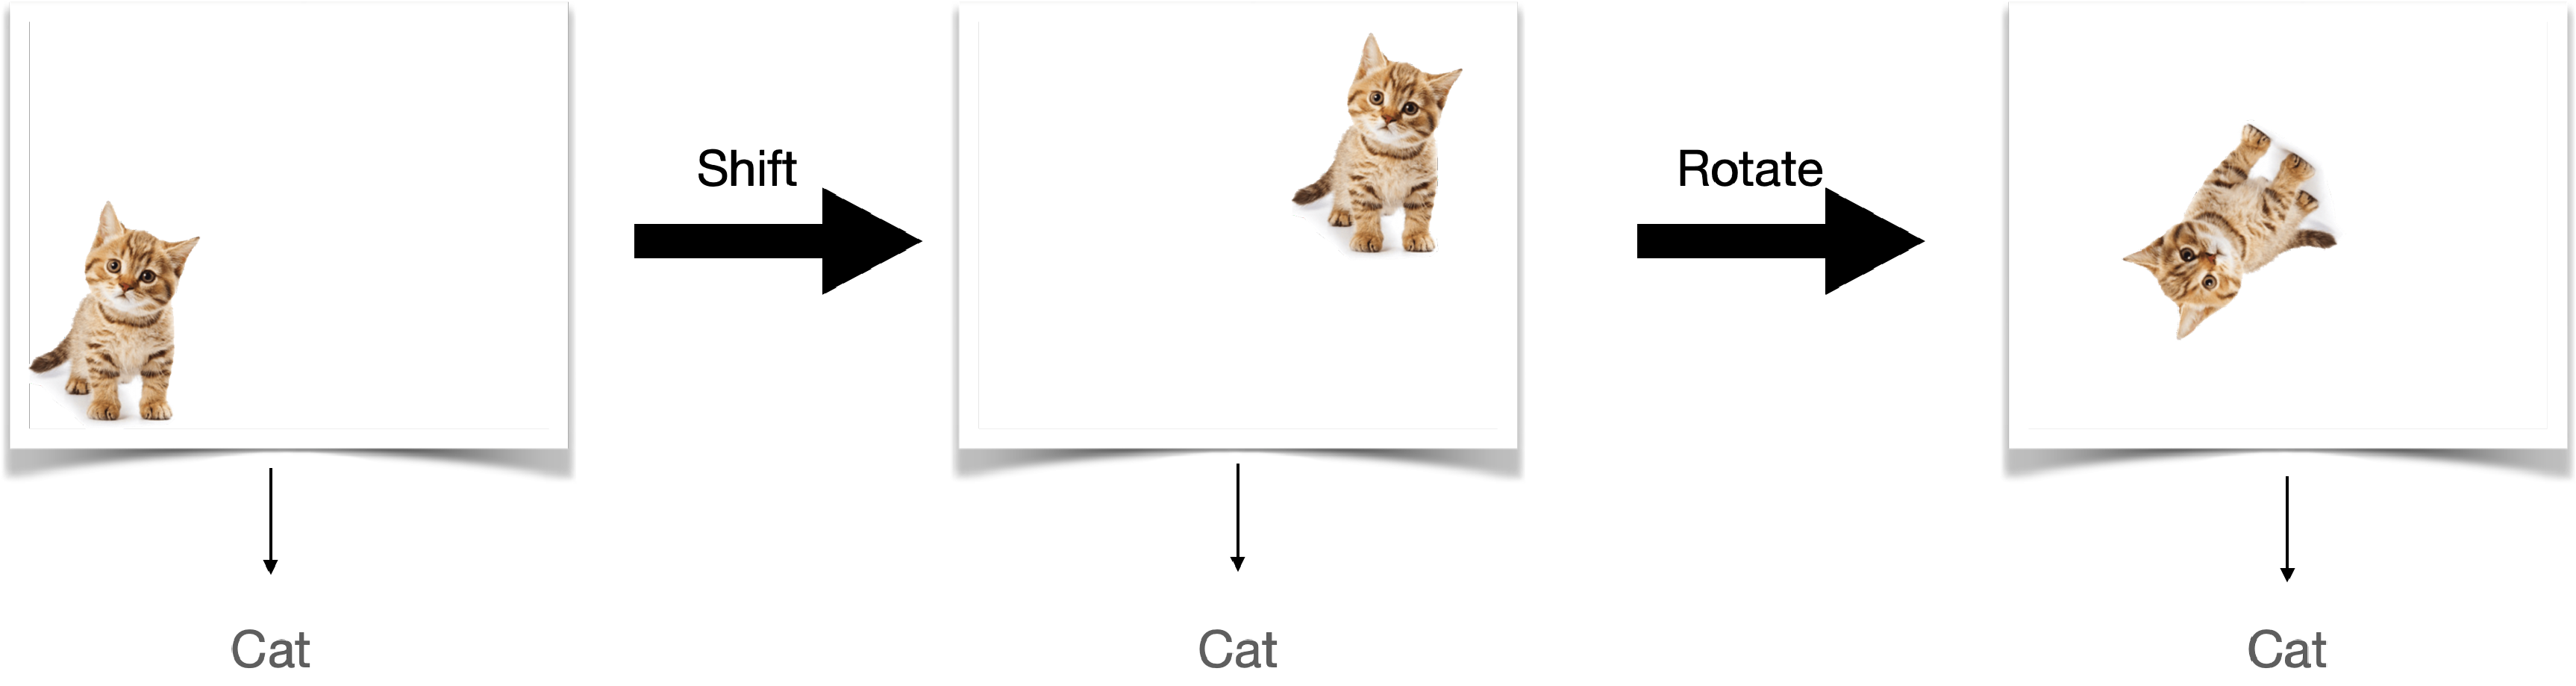
\includegraphics[width=0.95\textwidth]{shift-cat-example.pdf}
  \caption{\label{fig:intro:shift-cat-example}In the image classication
    task, we hope the learned model can still recognize \tquoted{cat} for the
    unseen image with shifted or rotated cat.}
\end{figure}

\subsubsection{Computer Vision Example: Shift-Invariant}
\label{sssec:intro:cv-example}

As the image classification task is shown
in~\autoref{fig:intro:shift-cat-example}, if a model is trained on the
first image with a cat in the bottom-left corner, we hope it can still
predict \tquoted{cat} when shift the cat to the upper-right corner.
Considering a feed-forward neural network, which can capture any
function, it may fail in this shifted case because not all the shifts
will exist in the training data. Augmenting the training data with the
shifted images may mitigate this problem. However, a more elegant way
is to use convolutional neural networks with a pooling layer. The
pooling operation over convolutional filters is largely
shift-invariant~\citep{zhang2019making}. Beyond the training data, the
inductive bias here assumes the model should be shift-invariant.
Similarly, on the third image
in~\autoref{fig:intro:shift-cat-example}, we also can assume the model
should be rotation-invariant to predict correctly on unseen rotated
cat images~\citep{cheng2016rifd}.

\begin{figure}[!tbp]
  \centering
  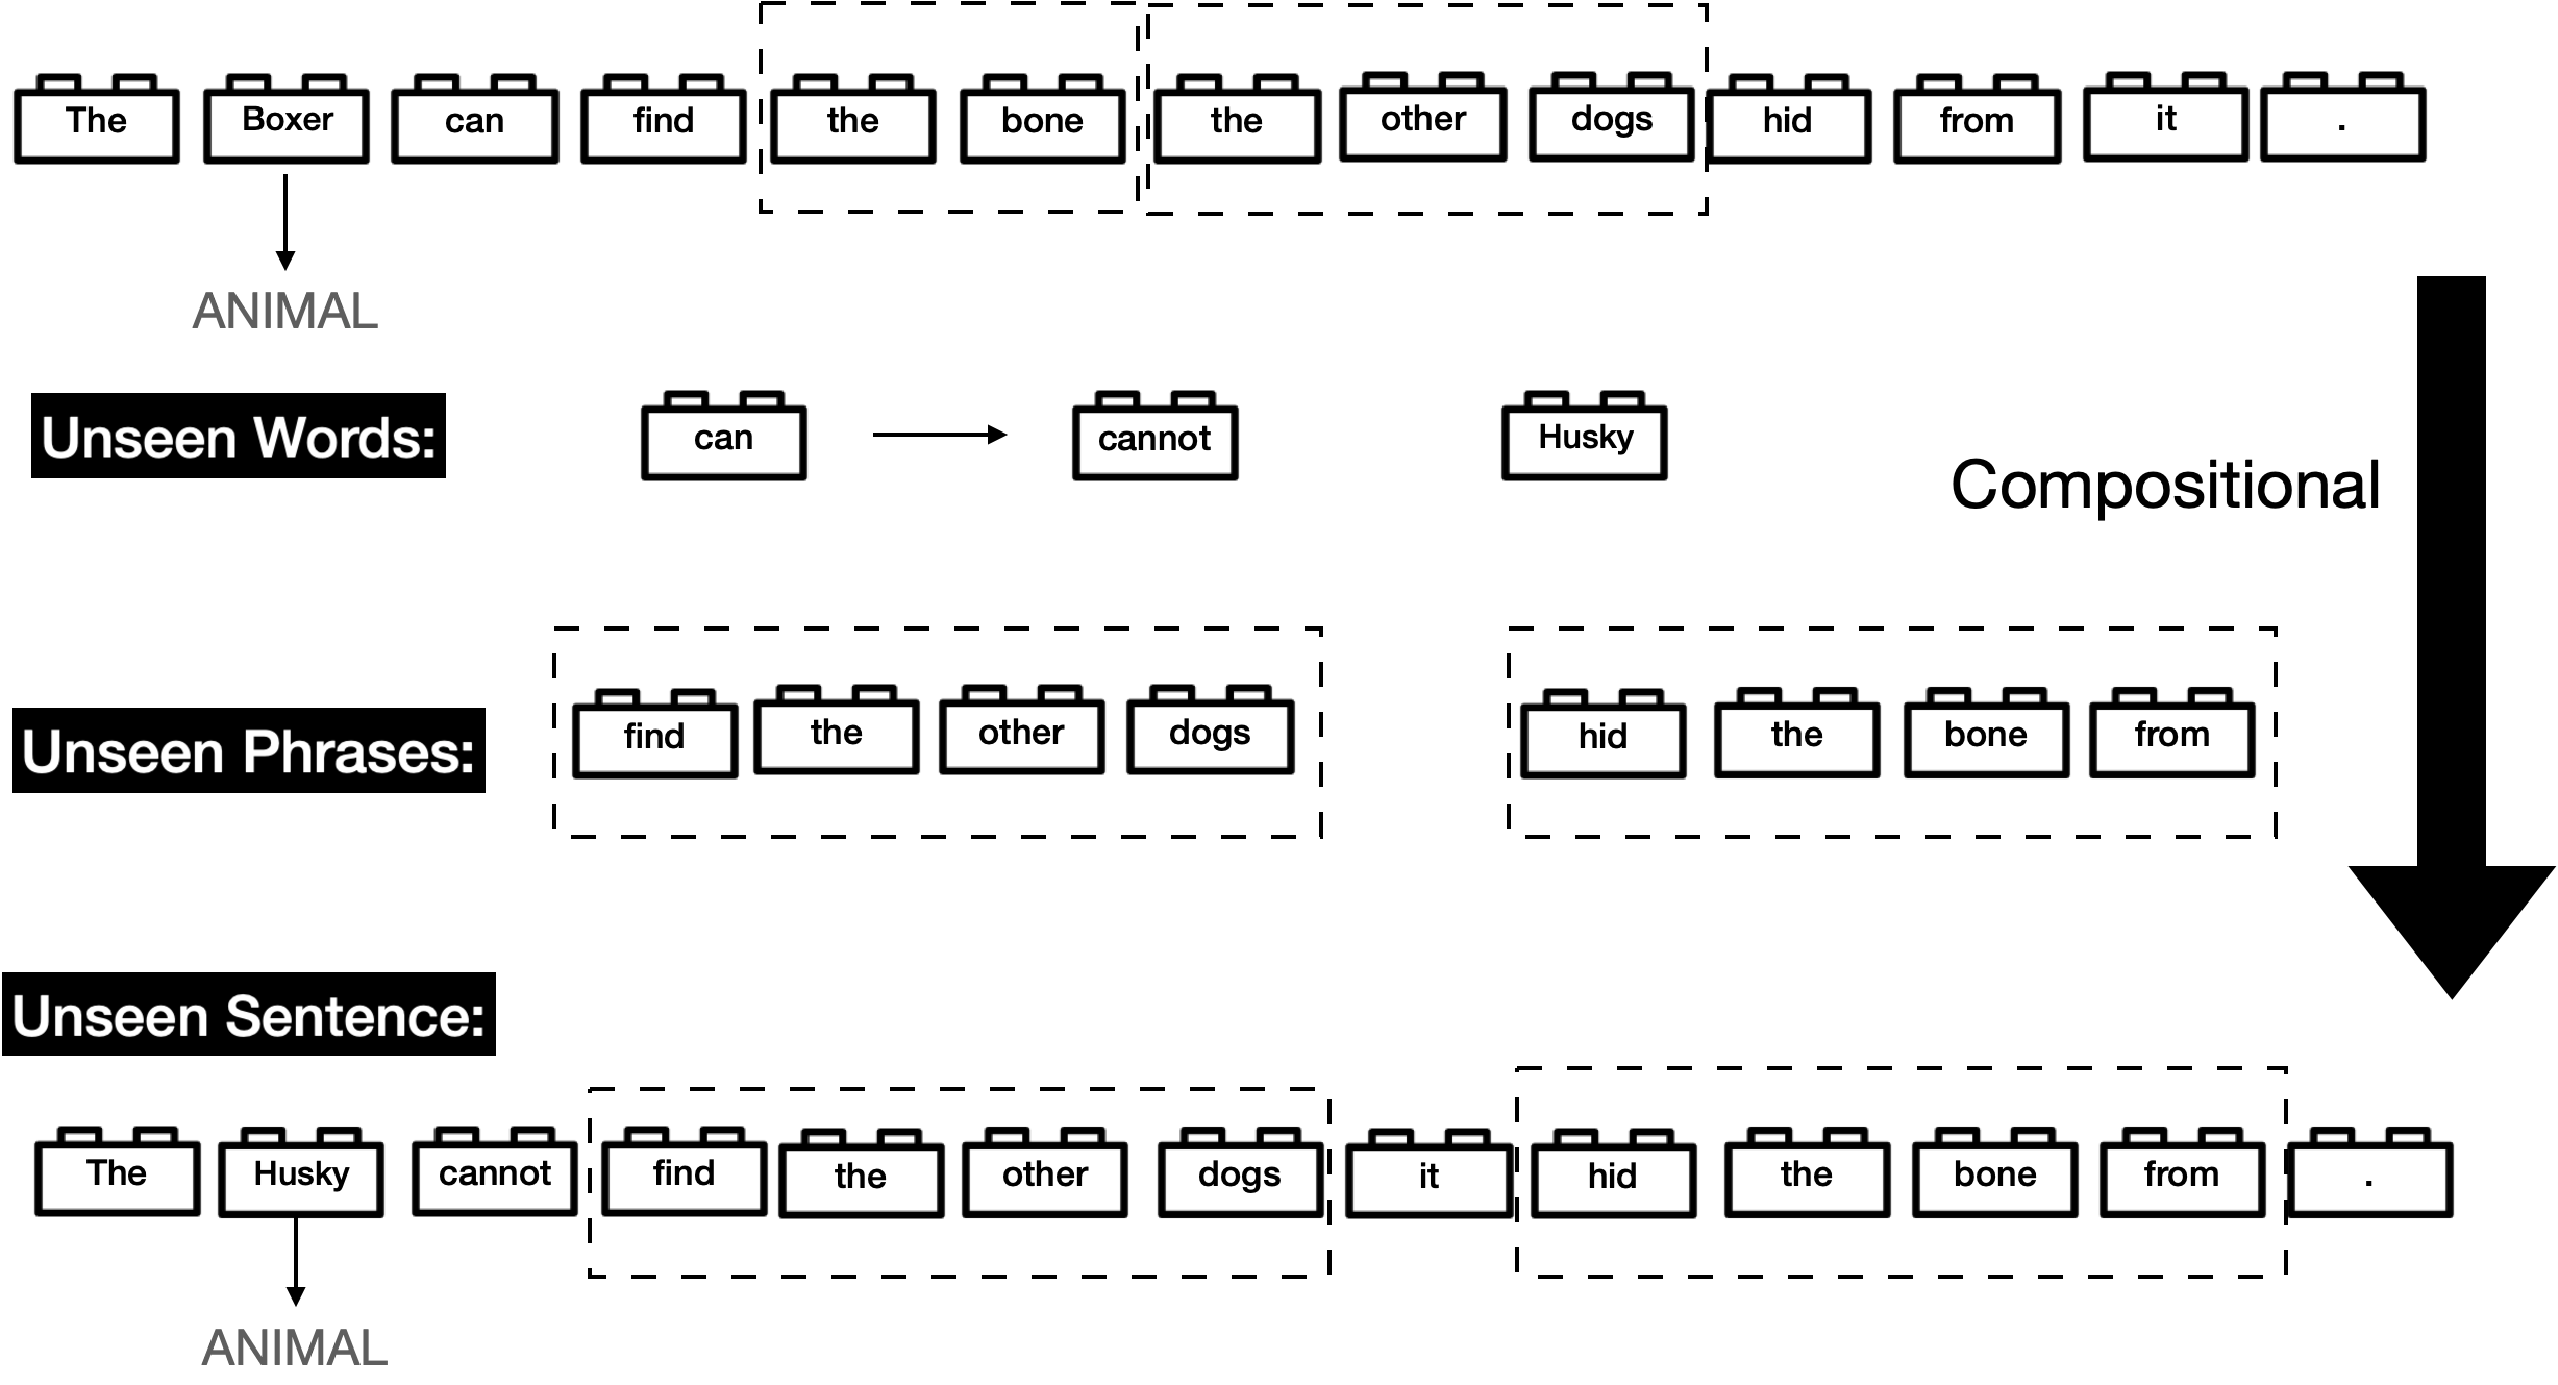
\includegraphics[width=0.98\textwidth]{compositional-dog-example.pdf}
  \caption{\label{fig:intro:compositional-dog-example}In the named entity
    recognization task, we hope the learned model can still recognize
    \tquoted{ANIMAL}~for new word~\tquoted{Husky} in unseen context with newly composed
    words, phases, and sentences.}
\end{figure}

\subsubsection{Natural Language Example: Compositionality}
\label{sssec:intro:nlp-example}

For natural language processing,
\autoref{fig:intro:compositional-dog-example} shows another example of
inductive biases in the named entity recognization task. Natural
language is naturally compositional. Beyond the training data, we
mainly make assumptions about the compositional properties for unseen
data. Imagining that the training data contains the first annotated
sentence:~\tquoted{The Boxer can find the bone the other dogs hid from
  it.}, here the word~\dquoted{Boxer} is annotated as~\tquoted{ANIMAL.}~Now
we add unseen new words, such as~\tquoted{cannot} and~\tquoted{Husky,}
and also add unseen new phrases by swapping the phrases~\tquoted{the
  bone}~and~\tquoted{the other dogs.} Finally, it forms an unseen new
sentence in the bottom of the figure. Can our model still predict the
unseen word~\tquoted{Husky}~in the unseen sentence as
\tquoted{ANIMAL}~?~We can augment the training data by enumerating
unseen combinations for the original training data. However, it is
intractable. To achieve this inductive bias about compositionality,
instead of augmenting all combinations, various techinique are
proposed to capture the underlying composing patterns inspired by
linguistic studies. For example, inspired by morphology study, word
piece~\citep{schuster2012japanese} and byte pair
encoding~\citep[BPE,][]{sennrich2016neural} may learn the
representation of unseen words, and they are widely used in the recent
advances in large language models, such as
BERT~\citep{devlin2019bert}, GPT3~\citep{brown2020language}. For
unseen phrases and sentences, inspired by the assumption about
recurrent syntax and grammar, recurrent neural networks~(such as
LSTM~\citep{hochreiter97lstm}, RNN~\citep{mesnil13rnn},
GRU~\citep{chung14gru}, and etc.)  are proposed to capture the
compositional patterns of natural language sequences. Instead of the
the strong recurrent assumption, a weaker word-order assumption also
works quite well by using a positional encoding with self-attention
mechanism in the popular transformer-based
models~\citep{NIPS2017_7181}. Finally, inspired by the distributional
hypodissertation, where words that are used and occur in the same contexts
tend to purport similar meanings~\cite{harris1954distributional},
bidirectional architectures are the standard for modeling word
embedding and language models.~(\eg, looking at both the past and
future via Bidirectional LSTM, self-attention, and so on)

Besides the shift-invariant, rotation-invariant and compositional
assumptions for the \kw{input} image and natural language data, there
are other assumptions beyond the training data that can be used in
deep learning era. In this dissertation, we extend the compositional
inductive biases for linguistic structured prediction
tasks.%\todo{SGD generalization,smoothness}
%\todo{Optimization will control the bias shift during learning}


%For example, naturally occurring data will often
%  underrepresent minority groups, so systems can do well on average
%  while having high error rates on these groups
%
% Datasets may also recapitulate stereotypes tied to historical
%%  injustices, which incentivizes models to learn these very
%  stereotypes to achieve the best test accuracy (Zhao et al., 2017,
%  2018; Rudinger et al., 2018). Training data collected from current
%  users of a system will likely be skewed towards users for which the
%  system works well, leading to a feedback loop in which underserved
%  users become increasingly underrepresented in the training data
%  (Hashimoto et al., 2018).
%\todo{Data augmentation for different pertubation}
%\todo{Realistic distribution shift}

\subsection[Independent Factorization for Deep Linguistic Structured
  Prediction]{Independent Factorization for Deep Linguistic \\Structured
  Prediction}
\label{ssec:intro:bias-dsp}

For systematic generalization, the search for appropriate inductive
biases is necessary for deep linguistic structured prediction.

First, beyond the compositionality of input natural language, we
believe that both the input text and output structured symbolic
representations will follow the principle of compositionality. The
composition of input natural language and the composition of output
representations are correlated with each other. Hence, we propose to
use the \kw{independent factorization} framework to study the
compositional inductive biases in natural language and its output
structures.

\subsubsection{Independent Factorization}
\label{ssec:intro:ind-factorization}

Let us denote an observation $x \in \mathcal{X}$. It can be any natural
language text, such as the sentence~\dquoted{The dog cannot find the
  bone it hid from the other dogs.} or a dialogue segment as shown
in~\autoref{fig:intro:dialogue}. We define an output structured
prediction for $x$ by $y \in \mathcal{Y}(x)$. Here $y$ is a structured
symbolic representation for $x$. For example, $y$ could be a sequence
of part-of-speech tags in~\autoref{fig:intro:dog-pos}, a constituent
tree in~\autoref{fig:intro:dog-tree} or a dependency tree
in~\autoref{fig:intro:dog-dep}. It can also be a broad-coverage
meaning representation, like AMR, UCCA, or a dialogue state table. To
represent the target function $y=f(x)$, we adopt the popular
energy-minimization strategy by defining $f(x)$ as the minimizer of an
auxiliary energy optimization problem.
\begin{equation}
\label{eq:argmin}
f(x) = \argmin_{y \in \mathcal{Y}(x)} E(x, y),
\end{equation}
where $E(x,y)$ is a scoring function representing the energy between
$x$ and a candidate output structure $y$.

In many NLP applications, the candidate output set $\mathcal{Y}(x)$ is
finite but exponentially large, and its size may depend on the input
$x$. For both exact and approximate optimization in
Equation~\ref{eq:argmin}, the main challenges lie on how to model the
representation of \IN~and~\OUT, and the interactions between
them. Practitioners typically employ energy functions with specific
factorization structures to design efficient algorithms, by assuming
the whole energy $E(x, y)$ can be decomposed as a sum of
\textbf{factors} $c$, denoted by $E(x, y) =\sum_{c \in C} E(x, y_{c})$.

A popular choice to represent the factorization is to index both $x$
and $y$ as a set of subcomponents $x=(x_{1},..., x_{i},.... x_{N})$
and $y=(y_{1},...y_{j},...y_{M})$. In AMR parsing as shown in
Figure~\ref{fig:intro:dog-amr}, $x_{i}$ can be a word or multiword
expression in a sentence, while $y_{j}$ can be a single AMR node and
relation.  For dialogue state tracking in
Figure~\ref{fig:intro:dialogue}, $x_{i}$ is an utterance in the
dialog, while $y_{i}$ is the value for each intent and slot in the
predicted frames. A factor $c$ may depend on multiple subcomponents
of $x$ and $y$.

The interdependence assumptions between those subcomponents in $x$
and $y$ are key in a structured prediction model. In the
\autoref{chap:background}, we show various representation formalism
~(such as graphical models), structured learning~(max-margin
framework) and inference approaches~(dynamic programming, integer
linear programming) to model interdependence. In this dissertation, we
always assume the \kw{independent factorization}, where each factor
$c$ only depends on a well-segmented subset of subcomponents $y_{c}$
and the aligned $x$ components~(anchors)~$x_{c}=a(y_{c})$. In other
words, once the output is decomposed into mutually exclusive output
segments, we consider each segment as an atomic output part, and each
atomic part is independent from the others.
\begin{equation}
    \label{eq:independent-factor}
    \begin{split}
    E(x, y) & =\sum_{c \in C} E(x, y_{c}) = \sum_{c \in C}E(x, a(y_{c}), y_{c})  \\
    \end{split}
\end{equation}
where $a(y_{c})$ is the alignment model to find how independent output
parts $y_{c}$ are \kw{anchored} to the constituents of the observation
$x$. Thus the prediction of each $y_{c}$ are independent from each
other, and can be locally decided by its aligned anchors.

Hence, this simple independent factorization can decompose the
structured learning into decomposed local learning~(still constrained
by some global constraints). In this way, independent factorization
largely simplifies the learning of linguistic structured
prediction. More importantly, it also makes the inference tractable,
and thus can be easily employed in the end-to-end neural network
training framework.

Using AMR parsing in~\autoref{fig:intro:dog-amr} as an example, the
independent factorization will first segment the output $y$ into small
parts $y_{c} \in seg_{out}(y)$, then find the anchors $x_{c}$ in the
input sentence for each $y_{c}$ from the candidate decomposition set
$seg_{in}(x)$. For example, one of the segmented $y_{c}$ in
Figure~\ref{fig:intro:dog-amr} is a precategorized subgraph
\tquoted{(possible-01 :polarity -),}~and its anchor $a(y_{c})$ is the
anchor word \tquoted{cannot.} The words \tquoted{the,} \tquoted{from}
are mapped to empty nodes.  Thus, by leveraging the compositionality
of the input and output, and the alignments between their
decompositions, we can focus on the prior knowledge about the
correlations between the input and output. Futhermore, we can extend
that compositionality to help the model to generalize to unseen inputs
and output structures.

\begin{figure}[!tbp]
\centering
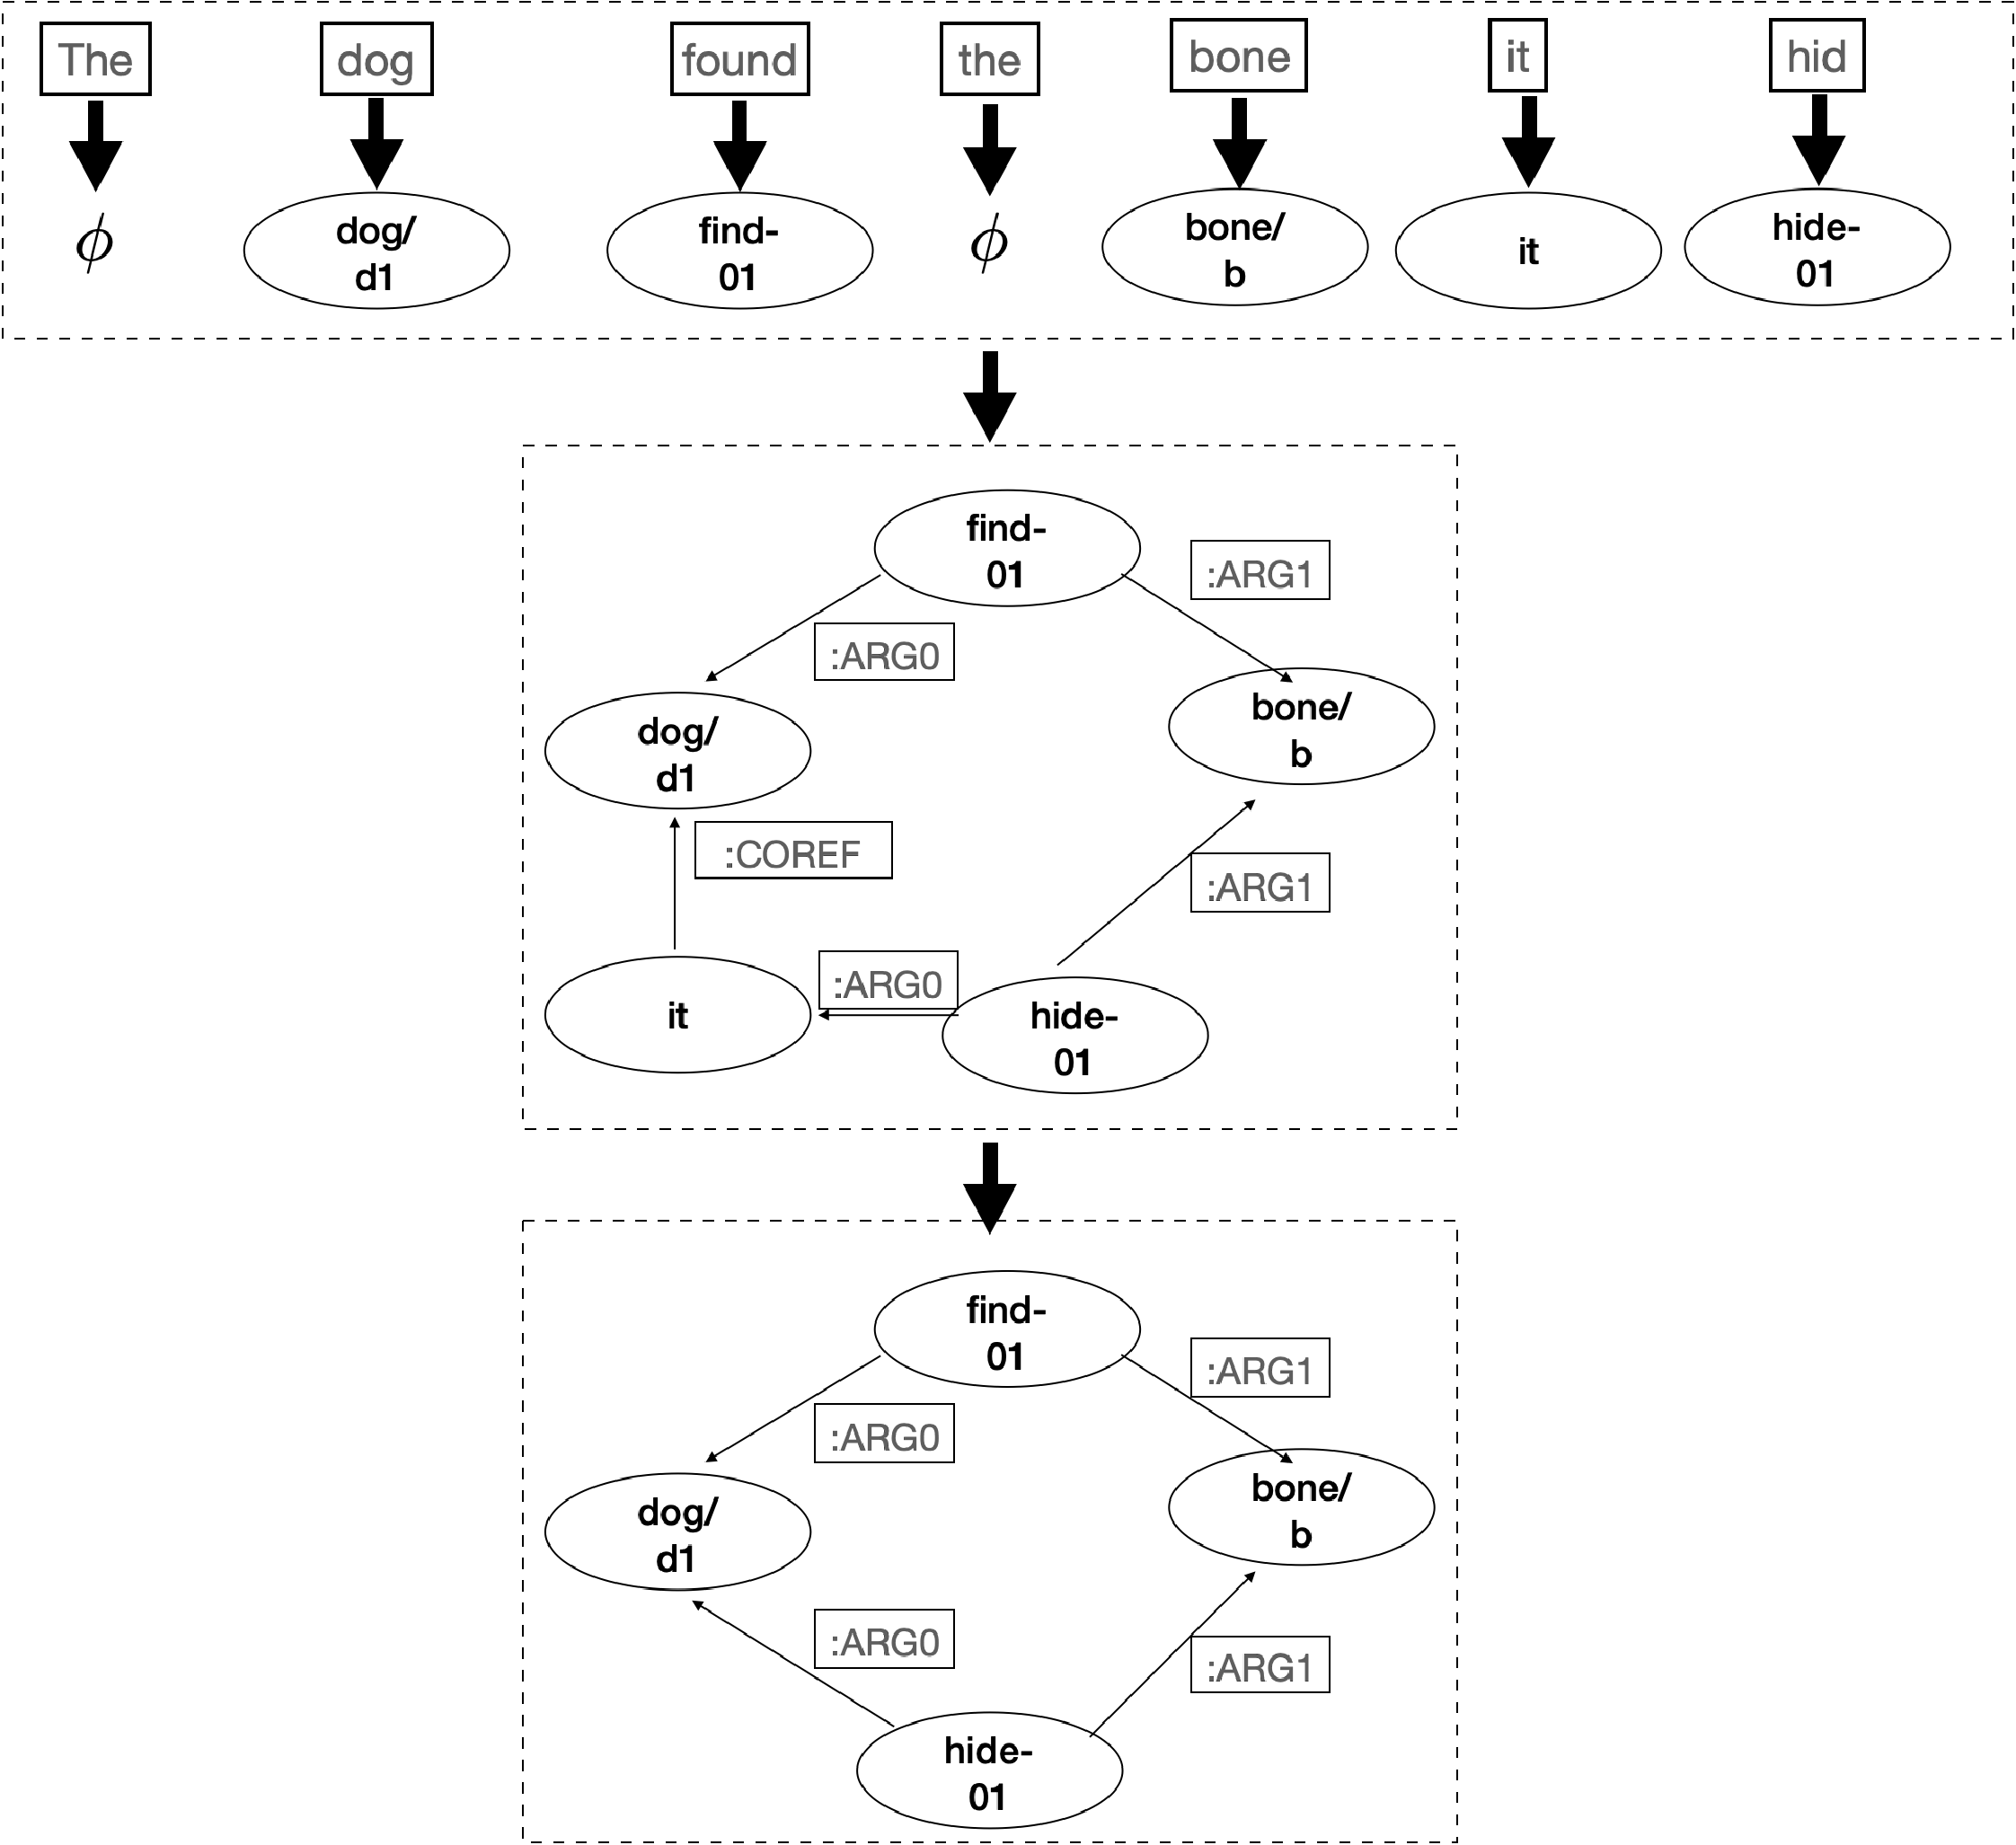
\includegraphics[width=0.80\textwidth]{dog-independent-example.pdf}
\caption{\label{fig:intro:independent-example}Independence
  factorization for parsing a new sentence \tquoted{The dog found the
    bone it hid} into an AMR graph.}
\end{figure}

During inference, when we encounter a new sentence as shown in
Figure~\ref{fig:intro:independent-example}, we hope the model can
leaverage the seen decomposed mappings in the training data to
generalize to the unseen sentences. In this way, we first prepare a
list of candidate anchors $seg_{in}(x)=\{${\tquoted{The},
  \tquoted{dog}, \tquoted{found}, \tquoted{the}, \tquoted{bone},
  \tquoted{it}, \tquoted{hide}$\}$, then the model will easily produce
  each independent prediction $y_{c}$ of each anchor as
  $\{\phi$,~\tquoted{dog},~\tquoted{find-01},~$\phi$,~\tquoted{bone},~\tquoted{it},~\tquoted{hide}$\}$
  because most of the decomposed inputs are seen in
  previous~\autoref{fig:intro:dog-amr}. Then we assemble the nonempty
  $y_{c}$ by predicting the relations between each other and finally
  forms \OUT~via postprocessing\footnote{The postprocessing include
    merging coreference nodes~(as the `dog' and `it'), and adding other
    attributes.}.

\subsubsection{Three Steps in Independent Factorizations}
\label{sssec:intro:steps-inductive-bias}
In summary, in the independence factorization setting, we factorize
the input and the output via the compositionality of both the input
and output, and then we hope the model can learn correlations between
the decomposed input and output parts. Hence, the whole structured
prediction problem is reduced into three challenges:

\begin{itemize}
\item \textbf{Output Decomposition:} How to decompose the output $y$
  into a set of independent parts $y_{c}$.

\item \textbf{Input Decomposition and Alignment Discovery:} How to decompose $x$ and offer a
  set of candidates that may generate each independent part $y_{c}$.
\item \textbf{Factor Modeling:} How to find the relevant parts
  $x_{a_{y_{c}}}$ in $x$ aligned to ${y_{c}}$ and model the factorized
  energy score $E(x, a(y_{c}), y_{c})$
\end{itemize}

The first question on independently decomposing $y$ is either
straightforward or has been resolved by previously existing methods in
our studied tasks. In this dissertation, we mainly focus on the remaining
challenges on modeling alignment and representation learning, which
requires different inductive biases to help with the
modeling. We consider the inductive biases to
help modeling the above structured correlations between the input and
output structures as \emph{structual inductive biases}, then we also
use \emph{natural language as inductive biases} to extend the
independent factorization for cross-domain and cross-task
generalization.

\subsubsection{Structural Inductive Biases}
\label{sssec:intro:structural-biases}
To design the independent factorization for a new task, we require the
prior knowledge about structures of input and output, \eg, proper
input decomposition, or the linguistic analysis on the
semantic-syntactic interface for the alignment information, or more
recent structural bias for deep learning based language modeling.

In this part, using the AMR parsing in
\autoref{fig:intro:structural-bias-example}) as a running example, we
consider the structural inductive biases for its independent
factorization. The first sentence and its corresponding AMR
graph~(left) are in training data, and we need to build a model to
predict the corresponding AMR graph for the unseen sentence. Hence, we
consider the compositionality for both the input and output to offer
more inductive biases beyond the training data. We leave more details
of AMR in \autoref{ssec:bg:amr} and more inductive biases about
decomposing AMR in
\autoref{sssec:lex-phr:lex-output-decomposition}. In this part, we
mainly show the intuitive understanding of the structural inductive
bias for the independent factorization.

\begin{figure}[!tbp]
  \centering
  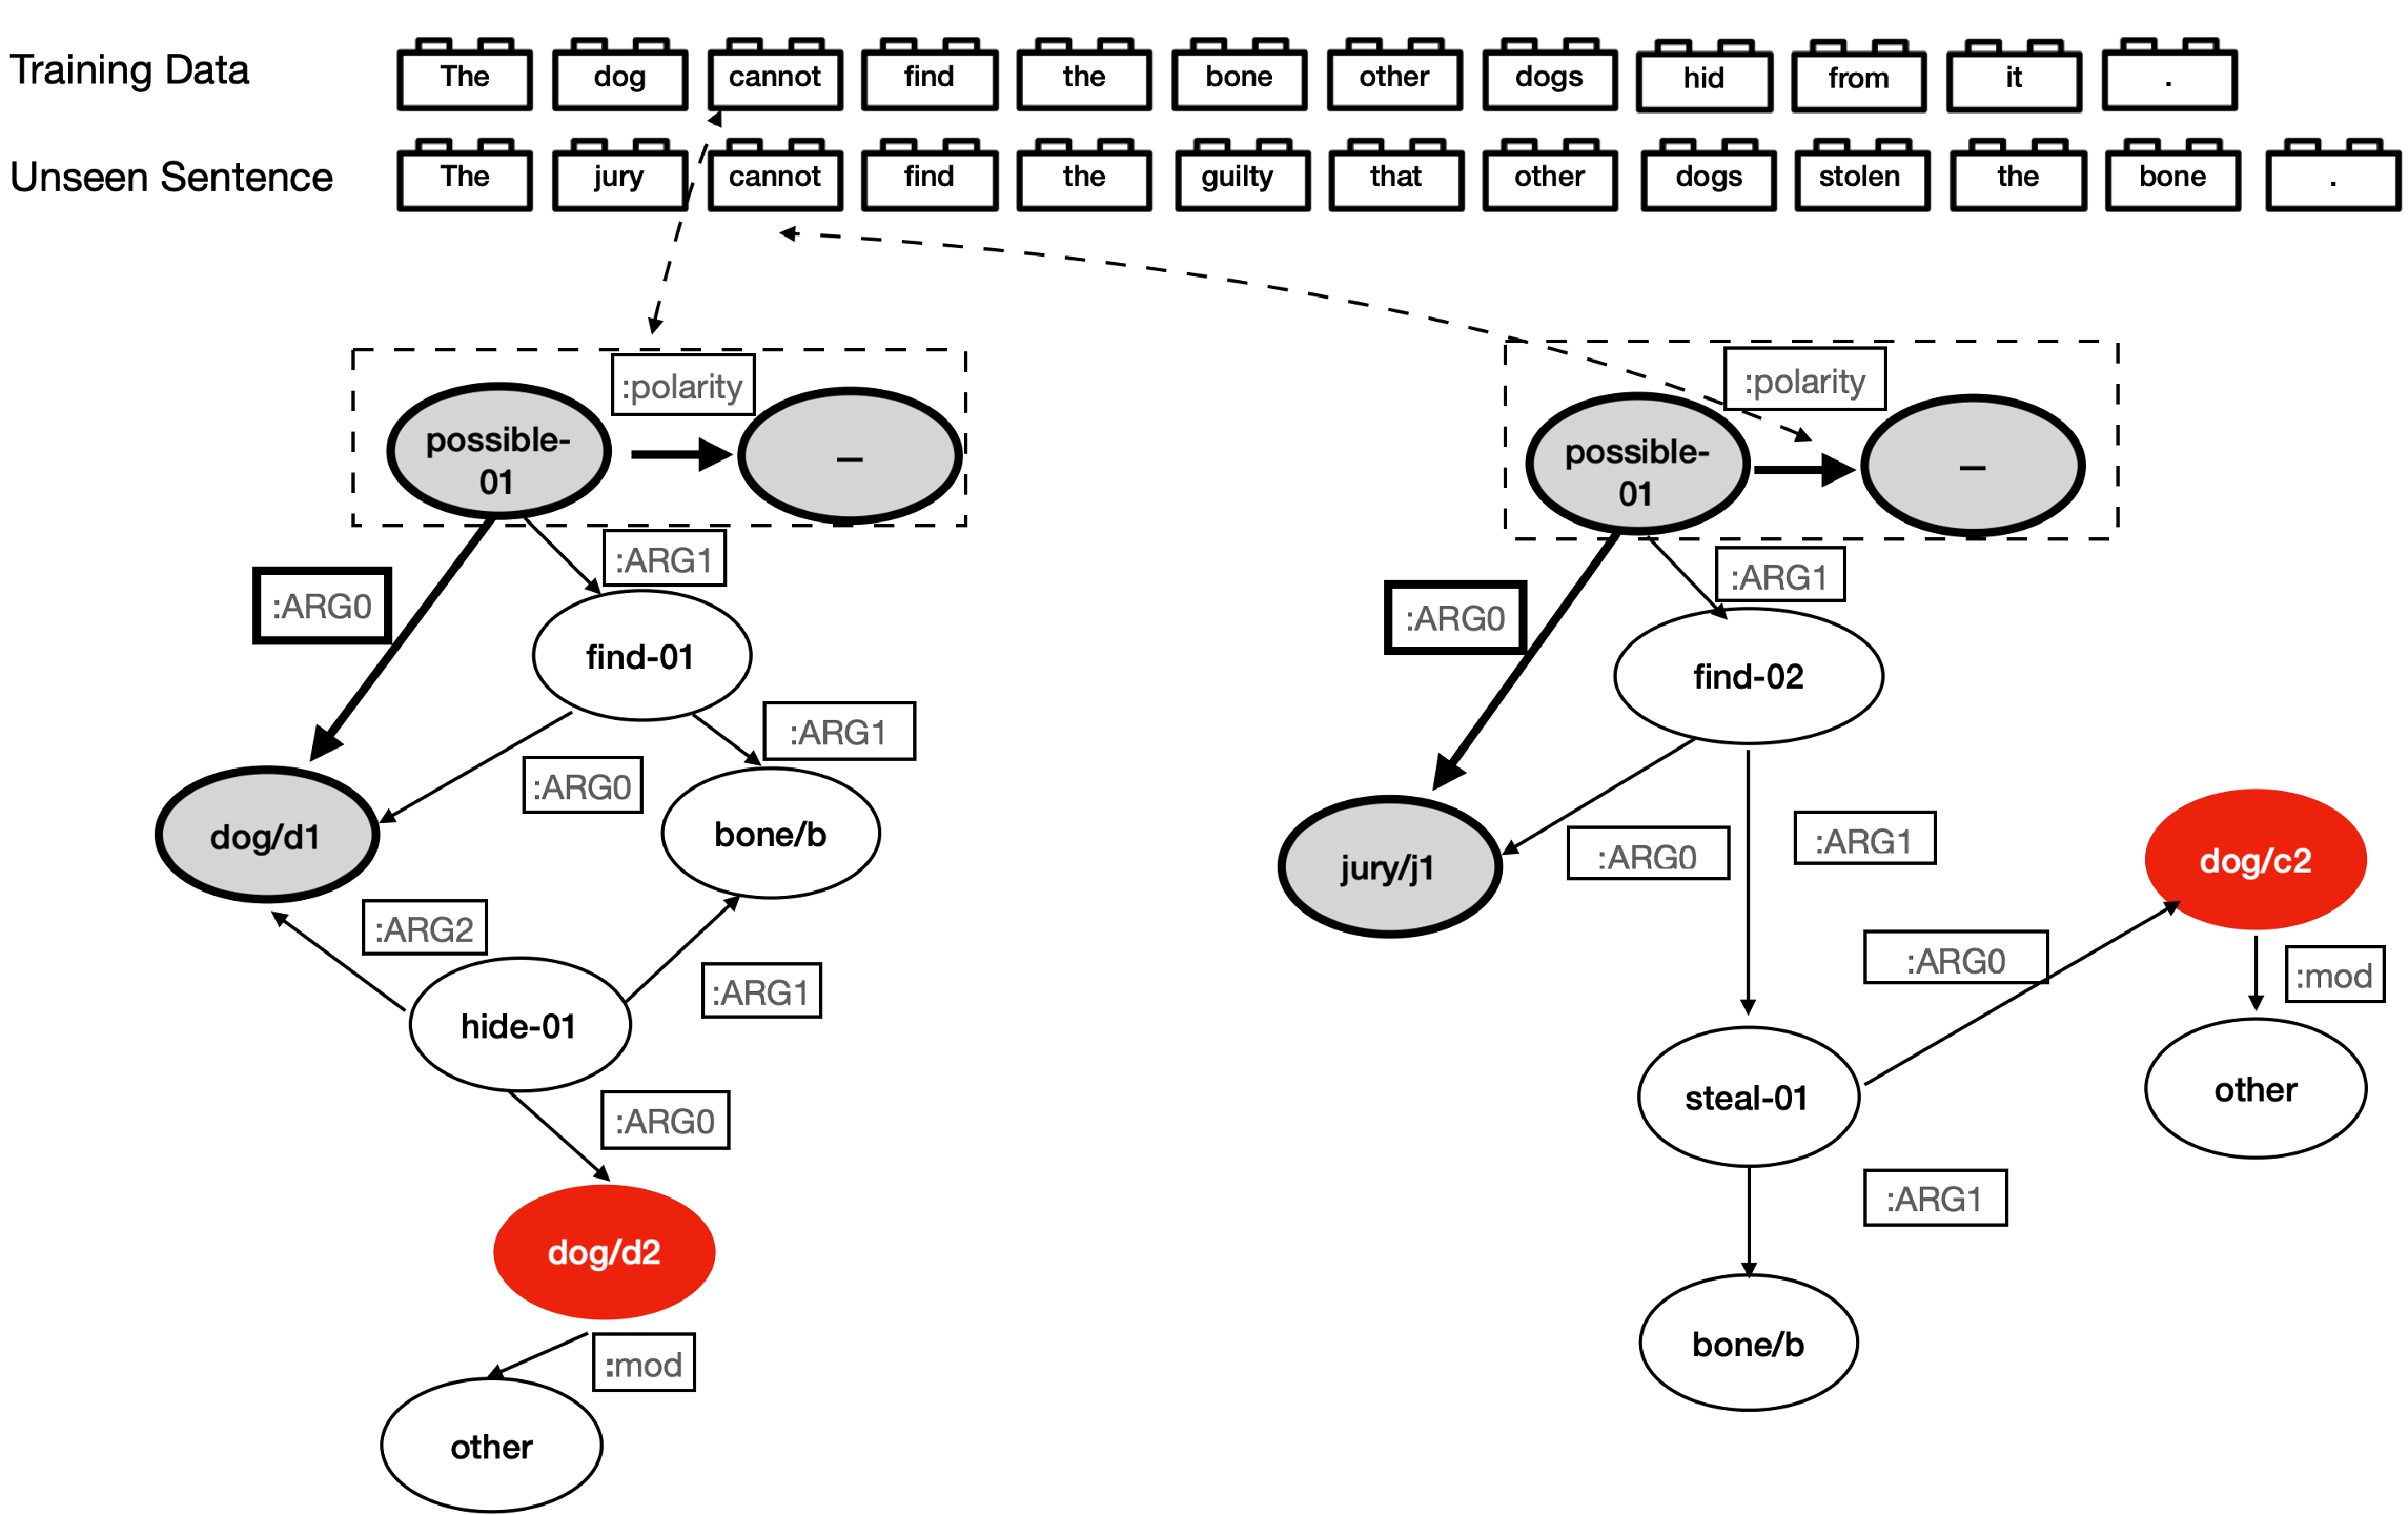
\includegraphics[width=0.95\textwidth]{structural-bias.pdf}
  \caption{\label{fig:intro:structural-bias-example} Structural inductive
    biases of AMR decomposition, and AMR alignments.}
\end{figure}

\begin{itemize}
\item \textbf{Output Decomposition:}~To decompose an AMR graph, we
  need to know the meaning of each part of the AMR graph. The nodes in
  AMR can be categorized into five main categories~(as shown in
  \autoref{fig:intro:structural-bias-example} and the example in later
  section~\autoref{ssec:bg:amr}): frame~(\eg, \tquoted{find-01,}
  \tquoted{hide-01}), basic concept~(\eg, \tquoted{dog,}
  \tquoted{jury}), string~(\tquoted{Pierre Vinken}), number~(\eg,
  \tquoted{61}) and other constant~(\eg, \tquoted{-}), while there
  many templated subgraphs used to represent special entities in the
  AMR, such as quantities, named entities, special roles, and other
  entities in dates, times, percentages, phone, email, URLs. In this
  part, we mainly show an example of subgraph segmentation for AMR,
  which will simplify the independent factorization. As shown in the
  left AMR graph, we draw a rectangle for the subgraph
  \tquoted{(possible-01 :polarity -),}~which means it forms a subgraph
  when decomposing the output AMR graph. The whole subgraph will be
  aligned to the word \tquoted{cannot} the first
  sentence. Furthermore, when there comes the second sentence, for the
  same word \tquoted{cannot} in the new sentence, we hope the model
  can produce the same subgraph \tquoted{(possible-01 :polarity -)}
  from it. Besides this subgraph, other segmented constituents in the
  left AMR graph will be each single node. While in other AMR graphs
  ~(\autoref{ssec:bg:amr}), we must consider the subgraphs used to
  represent the special entities. According to the above knowledge
  about the AMR graph, we use rule-based recategorization
  preprocessing to do the segmentation, which is inspired by the
  previous work on addressing the data sparsity issue in AMR
  parsing~\citep{Werling:2015up,foland-martin-2017-abstract,Wang:2017vt,Peng:2017ud}

\item \textbf{Input Decomposition and Alignment Discovery:}~As shown
  in the first row of Lego blocks in
  \autoref{fig:intro:structural-bias-example}, it naturally forms the
  decomposition of the first sentence for the AMR parsing
  case. However, for a more complicated case in~\autoref{ssec:bg:amr},
  rather than each standalone token, we may still need to consider
  other multiword expressions and the special entities in the
  sentence. Furthermore, when considering the previous UCCA parsing
  example shown in~\autoref{fig:intro:dog-ucca}, we also need to
  decompose the input sentence into phrases so that it can be easily
  aligned to the nonterminal nodes in the decomposed UCCA graph.
  Another problem after the input decomposition is the alignment
  discovery problem. We can notice two \tquoted{dog}~lego blocks in
  the first sentence, and we also have two \tquoted{dog}~AMR nodes. We
  have the words~\tquoted{from}~in the sentence. However, it cannot
  align to any node, the AMR nodes. We need to build an alignment
  model to distinguish the alignments between them. In sum, we must
  consider the input decomposition with the inductive biases on the
  semantic contents in the symbolic representations and how they are
  derived from the surface tokens.

\item \textbf{Factor Modeling:}~The above output and input
  decomposition are usually done with prior knowledge about the
  language and the corresponding symbolic representations. Once we get
  the segmented nodes or subgraphs for output decomposition and the
  Lego blocks as the input decomposition, the whole structured
  prediction problem is simplified to learning a set of models. For
  example, we hope the model can map the words~\tquoted{cannot} into
  the subgraph~\tquoted{(possible-01 :polarity -),}~and map \tquoted{hid}
  into \tquoted{hide-01.} When there is explicit alignment
  information, it will be easy to model them with aligned input and
  output pairs. However, when there are uncertainties about the
  alignments, we may need to model the alignment discovery model with
  the factor modeling jointly. We propose a latent alignment model for
  AMR parsing in~\autoref{sec:lex-phr:graph-based}. Besides that,
  considering the same word \tquoted{find} in both sentences, we need
  a discriminative contextualized representation to predict the
  correct meaning representation as the~\tquoted{find-01} for the
  first sentence and the~\tquoted{find-02} for the second
  sentence. The efficient contextualized representation is also the
  key to making such independent factorization possible. We will
  introduce more details of the two-stage AMR parsing
  in~\autoref{sec:lex-phr:graph-based}, which introduces how to
  assemble those local decisions about nodes and edges into a graph.
\end{itemize}

In sum, although the independent factorization simplifies structured
prediction into simpler classification problems, however, we need many
inductive biases to make the right design choices. Besides the above
AMR parsing running example, we also design different models with
independent factorization for a set of tasks, e.g., parsing
graph-based representations with
lexical-anchoring~(\autoref{ssec:lex-phr:lex-factorization-analysis})
and
phrasal-anchoring~(\autoref{ssec:lex-phr:phr-factorization-analysis}),
observing dialog in therapy~(\autoref{sec:snt:task}).

\subsubsection{Natural Language as Inductive Biases}
\label{sssec:intro:language-biases}
We also study natural language description as inductive biases to
describe the function of each decomposed output part. We still take
the AMR Parsing in \autoref{fig:intro:structural-bias-example} as a
running example. When we don't know the meaning of ~\tquoted{find-01}
and~\tquoted{find-02,}~to make the word~\tquoted{find} in the second
sentence can generate the~\tquoted{find-02} instead
of~\tquoted{find-01,}~it still needs a lot of aligned pairs about
the~\tquoted{find} from other training data to learn. This is true for
both human and machines. However, if we look at the explanation
of~\tquoted{find-01} and \tquoted{find-02} in
PropBank~\citep{Kin:Pal:02}, we may easily find that \tquoted{find-01}
means discovery, while \tquoted{find-02} means verdict. Hence, human
now can easily tell that the second~\tquoted{find} should
predict~\tquoted{find-02} because it means~\tquoted{verdict} by the
jury, without any more examples about~\tquoted{find-02.}~Once we know
the explanation of~\tquoted{find-01} and~\tquoted{find-02,}~we can
disambiguate them because we understand the meaning of the natural
language that is used for the explanation. We believe that the
knowledge in the natural language can also be used as inductive biases
for machine learning. In this dissertation, we mainly extend the independent
factorization of task-oriented dialogue state tracking with natural
language descriptions~(\autoref{chap:sgd}). We show that natural
language as inductive provides great zero-shot performance on unseen
dialogue services.

In sum, motivated by the compositional property of natural language
and related symbolic representation, we propose to use independent
factorization to model the correlations between the input and output
structures. Furthermore, to make the independent factorization work
for our models, we present a detailed analysis of how to do it for
each task, and how to use the above inductive biases to help model the
independent factorization.

%%% Local Variables:
%%% mode: latex
%%% TeX-master: "../../dissertation-main.ltx"
%%% End:
